%%!Mode:: "Tex:UTF-8"


\chapter{集中式事件激发采样下带部分未知转移率和时滞的复杂网络同步问题}
    上一章节讨论了基于分散式事件激发采样控制策略下的转移概率已知的马氏切换的复杂网络. 尽管网络模型考虑的切换拓扑的情形, 但是马氏链的转移率是已知的. 特别是多切换拓扑的模型中, 很难去精确获得每个切换拓扑间的转移率. 本章节将切换拓扑的转移率推广到部分未知的情形. 另一方面, 在现实的网络中, 由于信号传输和信息过程的有限速度以及有限带宽, 所以时滞是不可避免的, 如无线通信网络中由于环境噪声等影响用户间的通信会出现时间延迟的情况. 时滞可能会降低网络的性能和稳定性. 在采样策略上, 本章采用集中式事件激发采样方法, 集中式事件激发采样只有一个激发规则, 所有节点都按照此规则更新. 其特点是花费较少的计算负荷. 但采样频率会较频繁.

    %因此迟滞复杂网络的同步问题已经越来越引起了许多学者们的注意, 并且已成为一个热点话题. 例如, Wang\upcite{M24}利用牵制控制方法研究了带有马氏切换的随机复杂网络同步问题; 随后Zhou\upcite{M23}在Wang的基础上通过脉冲控制和牵制控制方法相结合, 给出了带马氏切换随机网络的簇同步判据; Yang\upcite{randomcoupling1}研究了非恒同节点时滞和随机耦合强度马氏切换复杂网络的同步问题. 尽管目前关于时滞已经积累了较多成果, 但是大部分的工作都只是没有考虑到随机环境的影响, 特别是切换拓扑, 即使有作者研究考虑了马氏切换情形, 但也是停留在马氏链转移概率全部已知的情况. 目前针对马氏链转移率部分未知的切换拓扑还没有相关成果, 跟不用说利用比较经济的事件激发策略去研究该类网络的同步问题. 除此之外, 同步目标有些情况下是通过节点之间相互协商才得出来的结果, 因此考虑动态的同步目标更具有使用价值.

\section{集中式事件激发采样的网络模型}

        在这一章节, 考虑一个部分未知转移率的马尔可夫链切换拓扑以及自身动力学时滞复杂网络, 在集中式事件激发采样控制策略下的数学模型如下:
        \begin{align}\label{sys:cen}
           \nonumber \dot{x}_{i}(t)&=f(t,x_{i}(t),x_i(t-\tau))-c\sum^N_{j=1}l_{ij}(r_{t})\Gamma[x_{j}(t_k)-x_{i}(t_{k})]+u_i(t),\\
            &\quad\quad t_{k}\leq t< t_{k+1}, \quad i = 1,\cdots,N,
        \end{align}
        这里的节点自身动力与前两章的模型相比较多了时滞因子, 即$f(\cdot,\cdot,\cdot): R\times R^n\times  R^n\mapsto  R^n$; $c$是常量耦合强度;
        $\{t_{1},t_{2},\cdots \}$是严格递增的激发时刻序列;
        $u_i(t)$是控制输入, 定义如下:
        \begin{align}\label{control}
            u_i(t)=-\rho c\beta_{i}(t)\frac{1}{N}\sum_{j=1}^N\Gamma[x_{i}(t_{k})-x_j(t_{k})],
        \end{align}
        这里$\rho c$是控制强度增益; $\beta_{i}(t)$是伯努利随机变量, 并且满足: $\mathrm{E}\beta_{i}(t)=\beta\in(0,1)$, $\mathrm{E}[\beta_{i}(t)\beta_{j}(t)]=\mathrm{E}\beta_{i}(t)\mathrm{E}\beta_{j}(t)$.
        \begin{rem}
            以上复杂网络模型除了马氏链和自身动力学与上一章不同之外, 该模型并不需要特定的同步目标轨道作为引导, 网络的同步目标是由节点在演变过程中确定的, 即这是一个动态调整的同步目标. 由于本节并未采用孤立节点的动力学行为作为网络同步目标, 而是采用动态协调的同步目标. 因此这里的控制输入的形式与上一章的控制形式有所不同. 每个节点的控制输入都是与该节点与其余节点的差成正比, 即根据节点自身与邻居节点之间的关系调整控制输入.
        \end{rem}

        由于自身动力学行为包含有时滞因子, 所以QUAD条件在本章不再适用, 下面给出类似Lipschitz条件的假设:
        \begin{hyp}{\rm\upcite{p29}}\label{ass1}
            对于节点自身动力学$f(\cdot,\cdot,\cdot)$, 假设存在两个常数$\alpha_1$和$\alpha_2$, 使得对任意的$x(t), y(t)\in R^n$, 有
         \begin{align*}
        \|f(t,x(t),x(t-\tau))-f(t,y(t),y(t-\tau))\|
        \leq\alpha_1\|x(t)-y(t)\|+\alpha_2\|x(t-\tau)-y(t-\tau)\|.
        \end{align*}
        \end{hyp}
    对于一些著名混沌吸引子, 例如蔡氏电路等, 他们的动力学$f(\cdot,\cdot,\cdot)$均满足上述假设. 在同步的文献中, 类似的假设已经被广泛地采用.

    下面给出本节至关重要的引理:
        \begin{lem}\label{mainlemma}
            如果半正定矩阵$A\in R^n$满足行和为零且有且仅有一个零特征根, 则对任意$x\in  R^n$, 只要$x^\top\mathbf{1}_N=0$, 则有$x^\top A x\geq\lambda_2x^\top x$, 其中$\lambda_2$是矩阵$A$最小非零特征值.
        \end{lem}
        \begin{proof}
        由于矩阵$A$是半正定矩阵且有且仅有一个零特征根, 所以将矩阵$A$的特征根进行如下排序: $0=\lambda_1<\lambda_2\leq\lambda_3\leq\cdots\leq\lambda_n$, 同时存在正交矩阵$P=(\xi_1,\xi_2,\cdots,\xi_n)$, $\xi_1=(1/\sqrt{n},1/\sqrt{n},\cdots,1/\sqrt{n})^\top$, $\xi_i\in R^n, i=1,2,\cdots,n$, 使得
        $A=PDP^\top$, 其中$D=\text{diag}\{\lambda_1,\lambda_2,\cdots,\lambda_n\}$. 又因为$A1_n=0$, 所以$(\lambda_11_n^\top\xi_1,\lambda_21_n^\top\xi_2,\cdots,\lambda_n1_n^\top\xi_n)\top=0$. 注意到$\lambda_i>0, i=2,\cdots,n$, 故 $\xi_i^\top1_n=0, i=2,\cdots,n$. 对任意向量$x\in  R^n$, $x^\top\mathbf{1}_N=0$, 存在向量$a=(a_1,a_2,\cdots,a_n)^\top\in R^n$ 使得$ x=Pa$. 根据$x^\top\mathbf{1}_N=0$以及$\xi_i^\top1_n=0, i=2,\cdots,n$, 可以得出 $a_1\xi_1^\top1_n=\sqrt{n}a_1=0$, 故$a_1=0$. 因此$x^\top A x=\lambda_2a_2^2+\lambda_3a_3^2+\cdots+\lambda_na_n^2\geq\lambda_2(a_2^2+a_3^2+\cdots+a_n^2)=\lambda_2a^\top a=\lambda_2x^\top x$.
        \end{proof}
        \begin{lem}[Halanay不等式]{\rm\upcite{delay-inq}}\label{Halanay}
            设$w(t)$ 是定义在区间$[t_0-\tau, \infty)$上的非负函数, 并且区间$[t_0, \infty)$上连续.
            如果存在两个正数$\xi$, $\eta$并且满足$\xi>\eta$, 使得
            $$\dot{w}(t)\leq -\xi w(t)+\eta w(t-\tau),\quad t\geq t_0,$$
            则$w(t)\leq w_{t_0}e^{-\gamma(t-t_0)}, t\geq t_0$,
            其中$w_{t_0}=\sup_{t_0-\tau\leq t\leq t_0}w(t)$, $\gamma>0$是方程$\xi-\gamma-\eta e^{\gamma\tau}=0$的最小实根.
        \end{lem}
        定义测量误差$\delta_i(t)=x_i(t_k)-x_i(t)$, 同步误差$e_{i}(t)=x_{i}(t)-s(t)$, 其中$s(t)=\frac{1}{N}\sum_{j=1}^Nx_j(t)$为参考节点.
        于是有${s}(t)=\frac{1}{N}(\mathbf{1}^\top_N\otimes I_n)x(t)$, 以及
        \begin{align}\label{reference}
        s(t)-s(t_k)&=\frac{1}{N}(\mathbf{1}^\top_N\otimes I_n)(x(t)-x(t_k))
        =-\frac{1}{N}(\mathbf{1}_N^\top\otimes I_n)\delta(t),
        \end{align}
        这里$x(t)=(x^\top_1(t),x^\top_2(t),\cdots,x^\top_N(t))^\top$, ${\delta}(t)=({\delta}^\top_1(t),{\delta}^\top_2(t),\cdots,{\delta}^\top_N(t))^\top$. 根据式 \eqref{control} 和式 \eqref{reference}, 可得
        \begin{align*}
        {u}_i(t)&=-\rho c\beta_i(t)\Gamma(x_i(t_k)-s(t_k))\\
        &=-\rho c\beta_i(t)\Gamma({\delta}_i(t)+x_i(t)-{s}(t)+{s}(t)-{s}(t_k))\\
        &=-\rho c\beta_i(t)\Gamma({\delta}_i(t)+e_i(t)-\frac{1}{N}(\mathbf{1}_N^\top\otimes I_n)\delta(t)).
        \end{align*}

        为了方便, 记$f(t,x(t),x(t-\tau))=(f^\top(t,x_1(t),x_1(t-\tau)),\cdots,f^\top(t,x_N(t),x_N(t-\tau)))^\top$, $B_t=\text{diag}\{\beta_{1}(t),\beta_{2}(t),\cdots,\beta_{N}(t)\}$. 由于$x_j(t_k)=\delta_j(t)+x_j(t)=\delta_j(t)+e_j(t)+s(t)$和$\sum_{j=1}^Nl_{ij}(r_t)=0$, 所以, 根据Kronecker积的性质, 式 \eqref{sys:cen} 可以被写成下式:
        \begin{align}\label{dxt}
        \nonumber \dot{x}(t)&=f(t,x(t),x(t-\tau))-c[L_{r_t}\otimes\Gamma]({\delta}(t)+e(t))\\
       &\quad-\rho c[B_t\otimes\Gamma][{\delta}(t)+e(t)-(U\otimes I_n)\delta(t)],\quad t_k\leq t<t_{k+1},
        \end{align}
        其中$U=\frac{1}{N}\mathbf{1}_N\mathbf{1}^\top_N$, $e(t)=(e^\top_1(t),\cdots,e^\top_N(t))^\top$. 因为$e(t)=x(t)-\mathbf{1}_N\otimes{s}(t)=x(t)-(U\otimes I_n)x(t)$ 和$(1_N^\top\otimes I_n)(L_{r_t}\otimes \Gamma)=(1_N^\top L_{r_t})\otimes \Gamma=0$, 所以网络系统 \eqref{sys:cen} 的误差系统为:
        \begin{align}\label{cee}
        \nonumber \dot{e}(t)&=\dot{x}(t)-(U\otimes I_n)\dot{x}(t)\\
        \nonumber&=f(t,x(t),x(t-\tau))-[U\otimes I_n]f(t,x(t),x(t-\tau))
        -c[L_{r_t}\otimes\Gamma]({\delta}(t)+e(t))\\
        \nonumber&\quad-\rho c[B_t\otimes\Gamma][{\delta}(t)+e(t)-(U\otimes I_n)\delta(t)]
        +\rho c[UB_t\otimes\Gamma][{\delta}(t)+e(t)-(U\otimes I_n)\delta(t)]\\
        \nonumber&=f(t,x(t),x(t-\tau))-[U\otimes I_n]f(t,x(t),x(t-\tau))
        -c[(L_{r_t}+\rho B_t-\rho UB_t)\otimes \Gamma]e(t)\\
        &\quad-c[(L_{r_t}+\rho B_t-\rho B_tU-\rho UB_t+\rho UB_tU)\otimes \Gamma]{\delta}(t),\quad t_k\leq t<t_{k+1}.
        \end{align}
\section{基于集中式事件激发采样的复杂网络同步分析}\label{result}
        下面设置集中式的事件激发策略, 结合随机发生控制的方法给出网络系统 \eqref{sys:cen} 的均方指数同步充分条件, 并且给出事件激发间隔的下界, 以确保在事件激发过程中不会发生事件瞬间累积, 即Zeno 现象. 在给出主要结论前, 先给出一些符号的说明: $\bar{\lambda}_v=\lambda_N(L_v)$, $\bar{\lambda}=\max_{u\in S}\{\lambda_N(L_u)\}$, $\lambda_2=\min_{u\in S}\{\lambda_2(L_u)\}$, $\gamma=\min_{i=1}^n\{\gamma_i\}$, $\bar{\gamma}=\max_{i=1}^n\{\gamma_i\}$.
\subsection{网络的同步判据}
        记$\hat{x}(t)=(L_{u}\otimes I_n)x(t)$, $\hat{{\delta}}(t)=(L_{u}\otimes I_n){\delta}(t)$, $\hat{e}(t)=(L_u\otimes I_n)e(t)$,  则有$\hat{e}(t)=(L_u\otimes I_n)e(t)=(L_{u}\otimes I_n)x(t)=\hat{x}(t)$. 定义事件激发函数如下:
        \begin{align}\label{trirule}
            g(t)=\|\hat{{\delta}}(t)\|-\varpi\|\hat{x}(t)\|,
        \end{align}
        其中$\varpi$是正数. 当事件激发函数达到阈值$0$时, 系统就会被激发, 激发时刻随即被确定, 即:
        \begin{align*}
            t_{k+1}=\max\{t\ge t_k: g(t)\le 0\}.
        \end{align*}
        \begin{thm}\label{them}
        如果假设$\ref{ass1}$成立, 并且存在常数$a,a_1,a_2,\cdots,a_m$, 使得对任意$u\in S$, 有:
            \begin{align}\label{thm:1}
            \left\{
            \begin{aligned}
            &\pi+a+\pi_u-c\gamma(\lambda_2+\rho\beta)\leq0,\\
            &2a\lambda_2^2-\bar{\lambda}\alpha_2>0,\\
            &L^2_v-a_uI_N\leq 0, \quad\quad \text{if} \quad v\neq u, v\in S_2^u, \\
            &L^2_v-a_uI_N\geq 0, \quad\quad \text{if} \quad v= u, v\in S_2^u,
            \end{aligned}
            \right.
            \end{align}
        其中$\pi=\bar{\lambda}(\frac{\alpha_1}{\lambda_2}+\alpha_2)$, $\pi_u=\frac{1}{2}\sum_{v\in S_1^u\setminus\{u\}}q_{uv}(\frac{\bar{\lambda}^2_{v}}{\lambda_2^2}-\frac{a_u}{\bar{\lambda}^2})
        +\frac{1}{2}q_{uu}I(u)(1-\frac{a_u}{\lambda_2^2})$, 如果$u\in S_1^u$, 则$I(u)=1$, 否则$I(u)=0$.
        那么, 在事件激发函数$(\ref{trirule})$下, 取$\varpi=\frac{c\gamma(\lambda_2+\rho\beta)-\pi-a-\max_{u\in S}\{\pi_u\}}{c\bar\gamma(\bar\lambda+\rho\beta)}$, 网络系统$(\ref{sys:cen})$对任意初值都可以实现均方指数同步.
        \end{thm}

        \begin{proof}
        定义随机Lyapunov-Krasovskii函数如下:
        \begin{align*}
        V(t)=\frac{1}{2}\hat{e}^\top(t)\hat{e}(t).
        \end{align*}
        记$x^k(t)=(x_1^k(t),x_2^k(t),\cdots,x_N^k(t))^\top$, $e^k(t)=(e_1^k(t),e_2^k(t),\cdots,e_N^k(t))^\top$, 则有:
        \begin{align}\label{ekt}
        \hat{e}^\top(t)\hat{e}(t)=e^\top(t)[L^2_u\otimes I_n]e(t)=\sum_{k=1}^ne^k(t)^\top L^2_ue^k(t).
        \end{align}
        因为$L_u$满足$\sum_{i=1}^Ne_i^k(t)=\sum_{i=1}^N[x_i^k(t)-\frac{1}{N}\sum_{j=1}^Nx_j^k(t)]=0$, 所以$L_ue^k(t)=0$当且仅当$e^k(t)=0$.
        因此$V(t)=0$当且仅当$e(t)=0$. 故Lyapunov-Krasovskii是合格的.

        根据式 \eqref{ekt} 和\autoref{mainlemma}, 有:
        \begin{align*}
        \hat{e}^\top(t)\hat{e}(t)=\sum_{k=1}^ne^k(t)^\top L^2_ue^k(t)\geq\lambda_2^2\sum_{k=1}^ne^k(t)^\top e^k(t)=\lambda_2^2e^\top(t)e(t).
        \end{align*}
        因此$\|\hat{x}(t)\|=\|\hat{e}(t)\|\geq\lambda_2\|e(t)\|$.

        因为$\mathrm{E}[B_t]=\beta I_N$和$L_uU=\frac{1}{N}L_u1_N1_N^\top=0$, 因此有:
        \begin{align}\label{sys:err}
        \nonumber \mathrm{E}\mathcal{L}V(t)&=\mathrm{E}\Big\{\hat{e}^{\top}(t)\dot{\hat{e}}(t)+\frac{1}{2}\sum_{v=1}^{m}q_{uv}\hat{e}^{\top}(t)\hat{e}(t)\Big\}\\
        \nonumber&=\mathrm{E}\Big\{\hat{e}^{\top}(t)[L_{u}\otimes I_n]f(t,x(t),x(t-\tau))
        -c\hat{e}^{\top}(t)[(L^2_u+\rho\beta L_u)\otimes \Gamma]e(t)\\
        &\quad-c\hat{e}^{\top}(t)[(L^2_u+\rho\beta L_u)\otimes \Gamma]{\delta}(t)
        +\frac{1}{2}\sum_{v=1}^{m}q_{uv}e^\top(t)[L^2_{v}\otimes I_n]e(t)\Big\}.
        \end{align}
        根据$L_u1_N=0$以及\autoref{ass1}, 有:
        \begin{align}\label{e1}
        \nonumber&\quad\mathrm{E}\Big\{\hat{e}^{\top}(t)[L_{u}\otimes I_n]f(t,x(t),x(t-\tau))\Big\}\\
        \nonumber &=\mathrm{E}\Big\{\hat{x}(t)[L_{u}\otimes I_n]\big[f(t,x(t),x(t-\tau))-\mathbf{1}_N\otimes f(t,{s}(t),{s}(t-\tau))\big]\Big\}\\
        \nonumber &\leq\mathrm{E}\Big\{\|\hat{x}(t)\|\|L_{u}\otimes I_n\|(\alpha_1\|e(t)\|+\alpha_2\|e(t-\tau)\|)\Big\}\\
        \nonumber &\leq\mathrm{E}\Big\{\bar{\lambda}\alpha_1\|\hat{x}(t)\|\|e(t)\|+\bar{\lambda}\alpha_2\|\hat{x}(t)\|\|e(t-\tau)\|)\Big\}\\
        \nonumber &\leq\frac{\bar{\lambda}\alpha_1}{\lambda_2}\mathrm{E}\|\hat{x}(t)\|^2+\bar{\lambda}\alpha_2(\mathrm{E}\|\hat{x}(t)\|^2+\frac{1}{2}\mathrm{E}\|e(t-\tau)\|^2)\\
        \nonumber &\leq\pi\mathrm{E}\|\hat{x}(t)\|^2+b\mathrm{E}V(t-\tau)\\
        &=-2a\mathrm{E}V(t)+b\mathrm{E}V(t-\tau)+(\pi+a)\mathrm{E}\{\hat{x}^\top(t)\hat{x}(t)\},
        \end{align}
        其中$\pi=\bar{\lambda}(\frac{\alpha_1}{\lambda_2}+\alpha_2)$, $b=\frac{\bar{\lambda}\alpha_2}{\lambda_2^2}$.
        通过利用\autoref{lem:2} 可得:
        \begin{align}\label{e13}
        \nonumber-c\mathrm{E}\Big\{\hat{e}^{\top}(t)[(L^2_u+\rho\beta L_u)\otimes \Gamma]e(t)\Big\}&=-c\mathrm{E}\Big\{\hat{e}^{\top}(t)[(L_u+\rho\beta I_N)\otimes \Gamma]\hat{e}(t)\Big\}\\
        &\leq-c\gamma(\lambda_2+\rho\beta)\mathrm{E}\{\hat{x}^{\top}(t)\hat{x}(t)\}.
        \end{align}
        根据范数三角不等式性可得:
        \begin{align}\label{e15}
        -c\mathrm{E}\Big\{\hat{e}^{\top}(t)[(L^2_u+\rho\beta L_u)\otimes \Gamma]{\delta}(t)\Big\}
        \nonumber&=-c\mathrm{E}\Big\{\hat{x}^{\top}(t)[(L_u+\rho\beta I_N)\otimes \Gamma]\hat{{\delta}}(t)\Big\}\\
        \nonumber&\leq c\mathrm{E}\Big\{\|\hat{x}^{\top}(t)\|\|(L_u+\rho\beta I_N)\otimes \Gamma\|\|\hat{{\delta}}(t)\|\Big\}\\
        &\leq c\bar{\gamma}(\bar{\lambda}+\rho\beta)\mathrm{E}\Big\{\|\hat{x}^{\top}(t)\|\|\hat{{\delta}}(t)\|\Big\}.
        \end{align}
        因为$\sum_{v=1}^{m}q_{uv}=0$, 结合条件 \eqref{thm:1}, 可得:
        \begin{align}\label{em}
        \nonumber&\quad\sum_{v=1}^{m}q_{uv}\mathrm{E}\Big\{e^\top(t)[L^2_{v}\otimes I_n]e(t)\Big\}\\
        \nonumber&=\sum_{v\in S_1^u}q_{uv}\mathrm{E}\Big\{e^\top(t)[(L^2_{v}-a_uI_N)\otimes I_n]e(t)\Big\}
        +\sum_{v\in S_2^u}q_{uv}\mathrm{E}\Big\{e^\top(t)[(L^2_{v}-a_uI_N)\otimes I_n]e(t)\Big\}\\
        \nonumber&\leq\sum_{v\in S_1^u\setminus\{u\}}q_{uv}\mathrm{E}\Big\{e^\top(t)[(L^2_{v}-a_uI_N)\otimes I_n]e(t)\Big\}
        +I(u)q_{uu}\mathrm{E}\Big\{e^\top(t)[(L^2_{u}-a_uI_N)\otimes I_n]e(t)\Big\}\\
        \nonumber&\leq\sum_{v\in S_1^u\setminus\{u\}}q_{uv}(\bar{\lambda}^2_{v}-a_u)\mathrm{E}\Big\{e^\top(t)e(t)\Big\}
        +I(u)q_{uu}\mathrm{E}\Big\{e^\top(t)[L^2_{u}\otimes I_n]e(t)\Big\}\\
        \nonumber&\quad-I(u)q_{uu}a_u\mathrm{E}\Big\{e^\top(t)e(t)\Big\}\\
        \nonumber&\leq\sum_{v\in S_1^u\setminus\{u\}}q_{uv}(\frac{\bar{\lambda}^2_{v}}{\lambda_2^{2}}-\frac{a_u}{\bar{\lambda}^{2}})\mathrm{E}\Big\{\hat{e}^\top(t)\hat{e}(t)\Big\}
        +q_{uu}I(u)(1-\frac{a_u}{\lambda_2^2})\mathrm{E}\Big\{\hat{e}^\top(t)\hat{e}(t)\Big\}\\
        &=2\pi_u\mathrm{E}\Big\{\hat{x}^\top(t)\hat{x}(t)\Big\},
        \end{align}
        其中$\pi_u=\frac{1}{2}\sum_{v\in S_1^u\setminus\{u\}}q_{uv}(\frac{\bar{\lambda}^2_{v}}{\lambda_2^2}-\frac{a_u}{\bar{\lambda}^2})
        +\frac{1}{2}q_{uu}I(u)(1-\frac{a_u}{\lambda_2^2})$, $I(u)$为示性函数, 即如果$u\in S_1^u$, 则$I(u)=1$, 否则$I(u)=0$.

        将式 \eqref{e1}$-$\eqref{em} 代入式 \eqref{sys:err}, 于是可得:
        \begin{align*}
        \mathrm{E}\mathcal{L}V(t)&\leq-2a\mathrm{E}V(t)+b\mathrm{E}V(t-\tau)+[\pi+a+\pi_u-c\gamma(\lambda_2+\rho\beta)]\mathrm{E}\Big\{\hat{x}^\top(t)\hat{x}(t)\Big\}\\
        &\quad+c\bar{\gamma}(\bar{\lambda}+\rho\beta)\mathrm{E}\Big\{\|\hat{x}^{\top}(t)\|\|\hat{{\delta}}(t)\|\Big\}.
        \end{align*}
        根据定理条件 \eqref{thm:1}, 当$t=t_k(k=1,2,\cdots)$时, 事件激发函数$g(t)=0$; 当$t_k<t<t_{k+1}, k=1,2,\cdots$时, 事件激发函数$g(t)<0$. 因此上式最后两项的和为非正数, 于是可得:
        \begin{align}\label{dEVt}
        \mathrm{E}\mathcal{L}V(t)\leq-2a\mathrm{E}V(t)+b\mathrm{E}V(t-\tau).
        \end{align}
        通过利用\autoref{Halanay}, 可得:
        \begin{align}\label{v0}
        \mathrm{E}V(t)\leq V_0e^{-\epsilon t},
        \end{align}
        其中$V_0=$ $\sup_{-\tau\leq t\leq0}\mathrm{E}V(t)$, $\epsilon>0$ 是方程$2a-\epsilon-\frac{\bar{\lambda}\alpha_2}{\lambda^{2}_2}e^{\epsilon t}=0$的最小实根. 根据$V(t)$的定义以及式 \eqref{v0}, 可得:
        \begin{align*}
        \mathrm{E}\|x_i(t)-{s}(t)\|^2\leq\frac{2}{\lambda^2_2}\mathrm{E}V(t)\leq\frac{2V_0}{\lambda_2^2}e^{-\epsilon t},\quad \forall i=1,\cdots,N.
        \end{align*}
        因此
        \begin{align*}
        \mathrm{E}\|x_i(t)-x_j(t)\|^2\leq\frac{8V_0}{\lambda_2^2}e^{-\epsilon t}, \quad\forall i,j=1,\cdots,N.
        \end{align*}
        根据 \autoref{defn1}, 网络系统 \eqref{sys:cen} 可以达到均方指数同步.
        \end{proof}
        \begin{rem}
        事实上, \autoref{them} 的条件是比较容易满足的. 首先, 选择合适的$a_u$使得最后两个不等式成立; 其次, 选择大于$\frac{\bar\lambda\alpha_2}{2\lambda_2^2}$ 的常数$a$; 最后, 选择合适的常数$c$和$\rho$就可以使得第一个不等式满足. 容易看出, 常数$c$和$\rho$在定理中扮演着重要的角色. 耦合强度$c$和控制强度$\rho$ 越大, 定理的条件就越容易满足. 即使节点间耦合强度$c$比较微弱, 但只要控制输入强度$\rho$足够大, 网络依然可以实现同步.
        \end{rem}
        \begin{rem}
        事件激发函数 \eqref{trirule} 只依赖于节点当前的状态信息和最新激发时刻的状态信息, 而不需要知道各个节点之间的差距或者是与虚拟同步目标之间的差距. $\|\hat{x}(t)\|$的系数$\varpi$是提前设计好的, 因此并不需要像Lu提出\upcite{eventsyn7}的激发规则那样在每次事件激发之后对该系数进行调整. 相比与Lu提出\upcite{eventsyn7}的激发规则, 事件激发函数 \eqref{trirule} 具有更低的计算复杂度.
        \end{rem}

        定理给出的结果是针对带有部分未知转移率的马尔可夫切换拓扑以及自身动力学存在时滞的网络模型, 对于更加简洁的模型有如下推论. 若马尔可夫链的转移率全部已知, 那么\autoref{them} 的条件可以被弱化.
        \begin{cor}
        如果假设$\ref{ass1}$成立, 并且存在常数$a>\frac{\bar{\lambda}\alpha_2}{2\lambda_2^2}$, 使得对所有$u\in S$, 有
            \begin{align*}
            &\pi+a+\pi_u-c\gamma(\lambda_2+\rho\beta)\leq0,
            \end{align*}
        其中$\pi=\bar{\lambda}(\frac{\alpha_1}{\lambda_2}+\alpha_2)$, $\pi_u=\frac{1}{2}\sum_{v\neq u}q_{uv}(\frac{\bar{\lambda}^2_{v}}{\lambda_2^2}-1)$.
        那么, 在事件激发函数 \eqref{trirule} 下, 取$\varpi=\frac{c\gamma(\lambda_2+\rho\beta)-\pi-a-\max_{u\in S}\{\pi_u\}}{c\bar\gamma(\bar\lambda+\rho\beta)}$, 网络系统 \eqref{sys:cen} 对于任意初值可以实现均方指数同步.
        \end{cor}
        若网络节点自身动力学不包含时滞, 并且马尔可夫链的转移率全部已知, 那么网络系统 \eqref{sys:cen} 可转化为:
        \begin{align}\label{cortwo}
          \nonumber \dot{x}_{i}(t)&=f(t,x_{i}(t))-c\sum^N_{j=1}l_{ij}(r_{t})\Gamma[x_{j}(t_k)
            -x_{i}(t_{k})]+u_i(t),\\
            &\quad t_{k}\leq t< t_{k+1} \quad i = 1,\cdots,N.
        \end{align}
        同时, \autoref{ass1} 变成常见的Lipschitz条件. 即, 假设存在常数$\alpha_1$使得对任意$x(t), y(t)\in  R^n$, 有
        \begin{align}\label{asss3}
        \|f(t,x(t))-f(t,y(t))\|\leq\alpha_1\|x(t)-y(t)\|.
        \end{align}
        \begin{cor}\label{cor2}
        如果$f(\cdot,\cdot)$满足条件 \eqref{asss3} 并且存在正数$a$, 使得对所有$u\in S$, 有
        \begin{align}\label{corcon2}
            \pi+a+\pi_u-c\gamma(\lambda_2+\rho\beta)\leq0,
        \end{align}
        其中$\pi=\frac{\bar{\lambda}\alpha_1}{\lambda_2}$, $\pi_u=\frac{1}{2}\sum_{v\neq u}q_{uv}(\frac{\bar{\lambda}^2_{v}}{\lambda_2^2}-1)$.
        那么, 在激发函数 \eqref{trirule} 下, 取$\varpi=\frac{c\gamma(\lambda_2+\rho\beta)-\pi-a-\max_{u\in S}\{\pi_u\}}{c\bar\gamma(\bar\lambda+\rho\beta)}$, 网络系统 \eqref{cortwo} 对于任意初值可以实现均方指数同步.
        \end{cor}
        \begin{rem}
        事实上, 网络系统$\eqref{cortwo}$与文Lu\upcite{eventsyn7}研究的系统是相类似的, 不同之处在于设置控制器时目标轨道的选取. 然而上述推论的条件更加容易满足. 这是由于条件$\eqref{corcon2}$是一般的实数不等式, 而Lu\upcite{eventsyn7}提出的定理条件是矩阵不等式. 除此之外, 本文事件激发规则更加简洁, 不需要在每次激发后更新激发函数的系数.
       \end{rem}
       若复杂网络耦合结构不受马氏链调制, 那么网络系统数学模型 \eqref{sys:cen} 改成下式:
        \begin{align}\label{sysnomarkov}
        \nonumber\dot{x}_{i}(t)&=f(t,x_{i}(t),x_i(t-\tau))-c\sum^N_{j=1}l_{ij}\Gamma[x_{j}(t_k)-x_{i}(t_{k})]+u_i(t),\\
           &\quad t_{k}\leq t< t_{k+1} \quad i = 1,\cdots,N.
        \end{align}
        \begin{cor}
        如果假设$\ref{ass1}$成立并且存在一个正数$a>\frac{\bar{\lambda}\alpha_2}{2\lambda_2^2}$, 使得:
           \begin{align*}
            \pi+a-c\gamma(\lambda_2+\rho\beta)\leq0,
            \end{align*}
        其中$\pi=\bar{\lambda}(\frac{\alpha_1}{\lambda_2}+\alpha_2)$.
        那么, 在事件激发函数 \eqref{trirule} 下, 取$\varpi=\frac{c\gamma(\lambda_2+\rho\beta)-\pi-a}{c\bar\gamma(\bar\lambda+\rho\beta)}$, 网络
        系统 \eqref{sysnomarkov} 对于任意初值可以实现均方指数同步.
        \end{cor}
\subsection{事件激发时刻间隔的下界}
        众所周知, 如果系统频繁地被激发, 那么将会出现不必要的事件累积, 即Zeno现象. 下面给出定理说明Zeno现象是不会出现的. 任意两次事件激发的时刻间隔都不会无限趋于零, 也就是说, 任意两个事件激发时刻间隔都存在正的下界.
        \begin{thm}\label{them2}
        如果假设$\ref{ass1}$成立, 并且存在常数$a,a_1,a_2,\cdots,a_m$, 使得对所有$u\in S$, 有
            \begin{align}\label{thm:2}
            \left\{
            \begin{aligned}
            &\pi+a+\pi_u-c\gamma(\lambda_2+\rho\beta)\leq0,\\
            &2a\lambda_2^2-\bar{\lambda}\alpha_2>0,\\
            &L^2_v-a_uI_N\leq 0, \quad\quad \text{if} \quad v\neq u, v\in S_2^u, \\
            &L^2_v-a_uI_N\geq 0, \quad\quad \text{if} \quad v= u, v\in S_2^u,
            \end{aligned}
            \right.
            \end{align}
        其中$\pi=\bar{\lambda}(\frac{\alpha_1}{\lambda_2}+\alpha_2)$, $\pi_u=\frac{1}{2}\sum_{v\in S_1^u\setminus\{u\}}q_{uv}(\frac{\bar{\lambda}^2_{v}}{\lambda_2^2}-\frac{a_u}{\bar{\lambda}^2})
        +\frac{1}{2}q_{uu}I(u)(1-\frac{a_u}{\lambda_2^2})$,如果$u\in S_1^u$, 则$I(u)=1$, 否则$I(u)=0$.
        那么, 在事件激函数$(\ref{trirule})$下, 取$\varpi=\frac{c\gamma(\lambda_2+\rho\beta)-\pi-a-\max_{u\in S}\{\pi_u\}}{c\bar\gamma(\bar\lambda+\rho\beta)}$, 对任意初值, 任意两个事件激发时刻间隔存在正的下界.
        \end{thm}
        \begin{proof}
        根据$\hat{{\delta}}(t)$的定义, 当$t=t_k$时, $\|\hat{{\delta}}(t)\|=0$; 当$t_k<t<t_{k+1}$时, $\|\hat{{\delta}}(t)\|<0$. $\|\hat{{\delta}}(t)\|$ 将会逐渐波动式增长, 直到它的值等于$\varpi\|\hat{x}(t)\|$时, 系统就会被激发. 也就是说, 事件间隔是$\frac{\|\hat{{\delta}}(t)\|}{\|\hat{x}(t)\|}$ 从$0$达到$\varpi$ 的时间段. 接下来寻找该段时间的一个正下界. 类似于D. Xie使用的方法\upcite{eventmult7}, 关键的问题是寻找函数$\frac{\|\hat{{\delta}}(t)\|}{\|\hat{x}(t)\|}$ 的上界函数. 注意到$\dot{\hat{{\delta}}}(t)=(L_{u}\otimes I_n)\dot{{\delta}}(t)=-(L_{u}\otimes I_n)\dot{x}(t)=-\dot{\hat{x}}(t)$, 因此有下面等式成立.
        \begin{align}\label{eet1}
        \frac{d\|\hat{{\delta}}(t)\|}{dt}=\frac{\hat{{\delta}}^\top(t)\dot{\hat\delta}(t)}{\|\hat{{\delta}}(t)\|}
        =\frac{\hat{{\delta}}^\top(t)(L_{u}\otimes I_n)\dot{\delta}(t)}{\|\hat{{\delta}}(t)\|}
        =\frac{-\hat{{\delta}}^\top(t)\dot{\hat{x}}(t)}{\|\hat{{\delta}}(t)\|}.
        \end{align}
        根据式 \eqref{eet1}, 有
         \begin{align}\label{ex}
        \nonumber\frac{d}{dt}\frac{\|\hat{{\delta}}(t)\|}{\|\hat{x}(t)\|}&=\frac{\|\hat{x}(t)\|}{\|\hat{x}(t)\|^2}\frac{d\|\hat{{\delta}}(t)\|}{dt}-\frac{\|\hat{{\delta}}(t)\|}{\|\hat{x}(t)\|^2}\frac{d\|\hat{x}(t)\|}{dt}\\
        \nonumber&=\frac{-\hat{{\delta}}^\top(t)\dot{\hat{x}}(t)}{\|\hat{{\delta}}(t)\|\|\hat{x}(t)\|}-\frac{\|\hat{{\delta}}(t)\|\hat{x}^\top(t)\dot{\hat{x}}(t)}{\|\hat{x}(t)\|^3}\\
   %     \nonumber&\leq\frac{\|\dot{\hat{x}}(t)\|}{\|\hat{x}(t)\|}+\frac{\|\hat{{\delta}}(t)\|\|\dot{\hat{x}}(t)\|}{\|\hat{x}(t)\|^2}\\
        &\leq\Big(1+\frac{\|\hat{{\delta}}(t)\|}{\|\hat{x}(t)\|}\Big)\frac{\|\dot{\hat{x}}(t)\|}{\|\hat{x}(t)\|}.
        \end{align}
        利用\autoref{ass1} 和式 \eqref{dxt} 可得:
        \begin{align}\label{eet0}
        \nonumber\|\dot{\hat{x}}(t)\|&=\|(L_{u}\otimes I_n)\dot{x}(t)\|\\
        \nonumber&=\Big\|(L_{u}\otimes I_n)\big[f(t,x(t),x(t-\tau))
        -c(L_{u}\otimes\Gamma)({\delta}(t)+e(t))\\
        \nonumber&\quad-c\rho(B_t\otimes\Gamma)({\delta}(t)+e(t)-(U\otimes I_n){\delta}(t))\big]\Big\|\\
        \nonumber&\leq\|(L_{u}\otimes I_n)f(t,x(t),x(t-\tau))\|+c\|(L(u)\otimes \Gamma)
        (\hat{{\delta}}(t)+\hat{e}(t))\|\\
        \nonumber&\quad+c\rho\|(I_N\otimes\Gamma)(\hat{{\delta}}(t)+\hat{e}(t))\|\\
        &\leq\frac{\bar{\lambda}\alpha_1}{\lambda_2^2}\|\hat{x}(t)\|+\frac{\bar{\lambda}\alpha_2}{\lambda_2^2}\|\hat{x}(t-\tau)\|
        +c\bar{\gamma}(\bar{\lambda}+\rho)(\|\hat{{\delta}}(t)\|+\|\hat{x}(t)\|).
        \end{align}
        将式 \eqref{eet0} 代入式 \eqref{ex}, 可得:
         \begin{align}\label{ex1}
        \frac{d}{dt}\frac{\|\hat{{\delta}}(t)\|}{\|\hat{x}(t)\|}&\leq\Big(1+\frac{\|\hat{{\delta}}(t)\|}{\|\hat{x}(t)\|}\Big)
        \Bigg[\frac{\bar{\lambda}\alpha_1}{\lambda_2^2}+\frac{\bar{\lambda}\alpha_2}{\lambda_2^2}\frac{\|\hat{x}(t-\tau)\|}{\|\hat{x}(t)\|}
        +c\bar{\gamma}(\bar{\lambda}+\rho)\Big(1+\frac{\|\hat{{\delta}}(t)\|}{\|\hat{x}(t)\|}\Big)\Bigg].
        \end{align}
        根据条件 \eqref{thm:2} 和\autoref{them}, $\lim_{t\rightarrow \infty}\|\hat{x}(t)\|=\lim_{t\rightarrow \infty}\|\hat{e}(t)\|=0$. 因此存在正数$\kappa$使得对所有$t>0$, $\frac{\|\hat{x}(t-\tau)\|}{\|\hat{x}(t)\|}\leq \kappa$成立. 故式 \eqref{ex1} 转化为:
        \begin{align}\label{ax2}
        \frac{d}{dt}\frac{\|\hat{{\delta}}(t)\|}{\|\hat{x}(t)\|}\leq c\bar{\gamma}(\bar{\lambda}+\rho)\Big(1+\frac{\|\hat{{\delta}}(t)\|}{\|\hat{x}(t)\|}\Big)^2
        +(\frac{\bar{\lambda}\alpha_1}{\lambda_2^2}
        +\frac{\bar{\lambda}\alpha_2}{\lambda_2^2}\kappa)\Big(1+\frac{\|\hat{{\delta}}(t)\|}{\|\hat{x}(t)\|}\Big).
        \end{align}
        记$k_1=c\bar{\gamma}(\bar{\lambda}+\rho)$, $k_2=\frac{\bar{\lambda}\alpha_1}{\lambda_2^2}
        +\frac{\bar{\lambda}\alpha_2}{\lambda_2^2}\kappa$.
        根据比较原理, $\frac{\|\hat{{\delta}}(t)\|}{\|\hat{x}(t)\|}\leq\phi(t,\phi_0)$, 其中$\phi(t,\phi_0)$是微分方程 $\dot{\phi}(t)=k_1(1+\phi(t))^2+k_2(1+\phi(t))$关于初值$\phi(0,\phi_0)=\phi_0$的解. 通过求解该微分方程可得:
        \begin{align}
        \phi(t)=\frac{k_2\exp\big\{k_2t+\ln\frac{k_1\phi_0+k_1}{k_1\phi_0+k_1+k_2}\big\}}{k_1-k_1\exp\big\{k_2t+\ln\frac{k_1\phi_0+k_1}{k_1\phi_0+k_1+k_2}\big\}}-1,
        \end{align}
        因此
        \begin{align}
        \frac{\|\hat{\delta}(t)\|}{\|\hat{x}(t)\|}\leq\phi(t).
        \end{align}
        从而, 任意两个事件激发$t_k$, $t_{k+1}$的时刻间隔的正下界$\tau^*$ 满足$\phi(\tau^*,0)=\varpi$. 通过求解该方程可得:
        $$\tau^*=\frac{1}{k_2}\ln\frac{(k_1+k_2)(1+\varpi)}{k_2+k_1(1+\varpi)}.$$
        即$\tau^*$使任意两个事件激发时刻间隔的下界.
        \end{proof}

\section{数值模拟}
    \begin{figure}
  % Requires \usepackage{graphicx}
     \begin{center}
            \subfigure[]{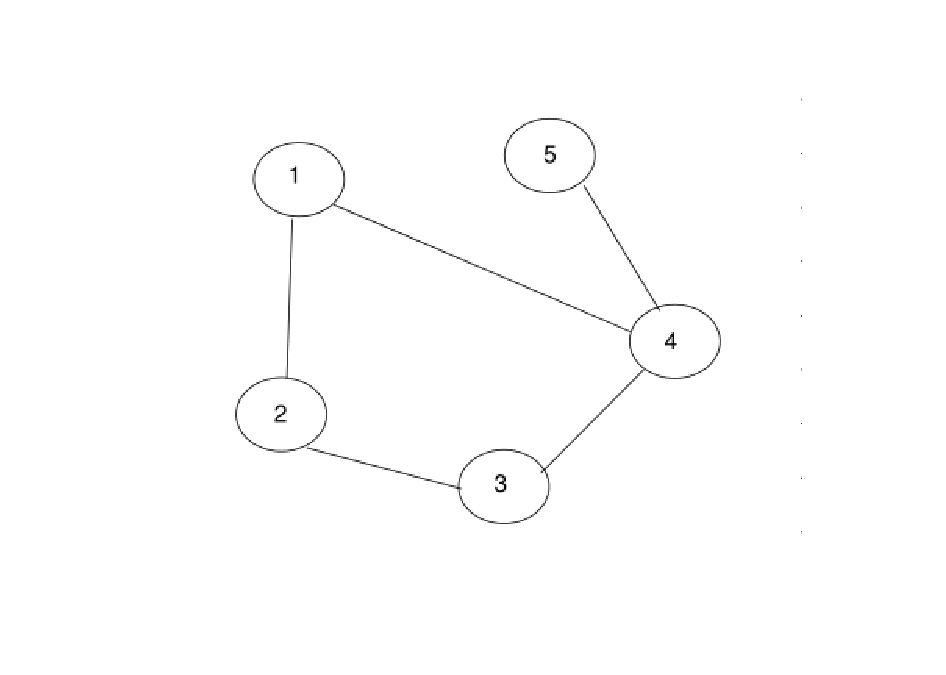
\includegraphics[width=1.8in]{delay/tuopu1.eps}}
            \subfigure[]{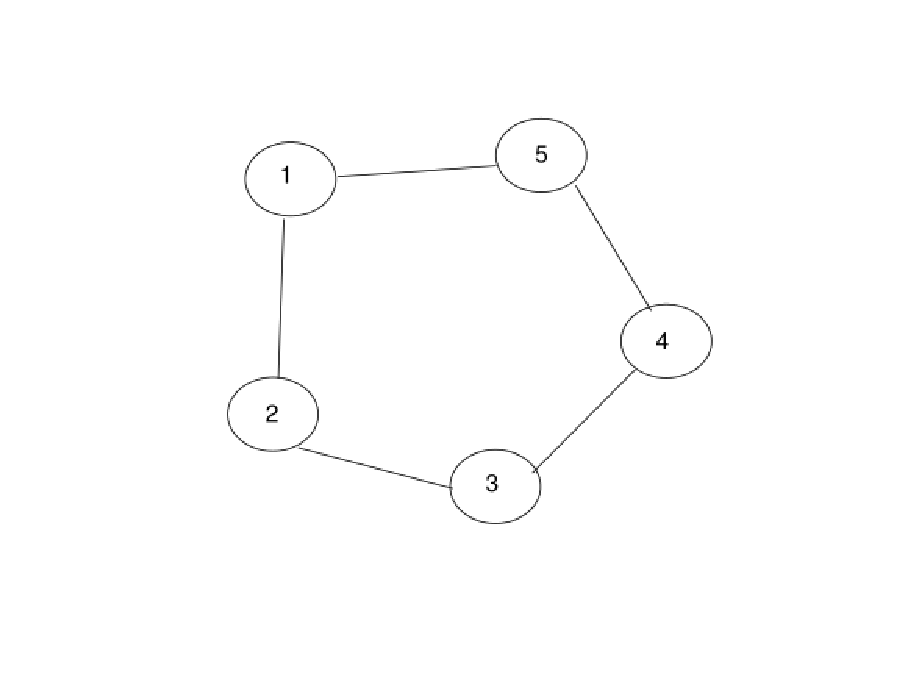
\includegraphics[width=1.8in]{delay/tuopu2.eps}}
            \subfigure[]{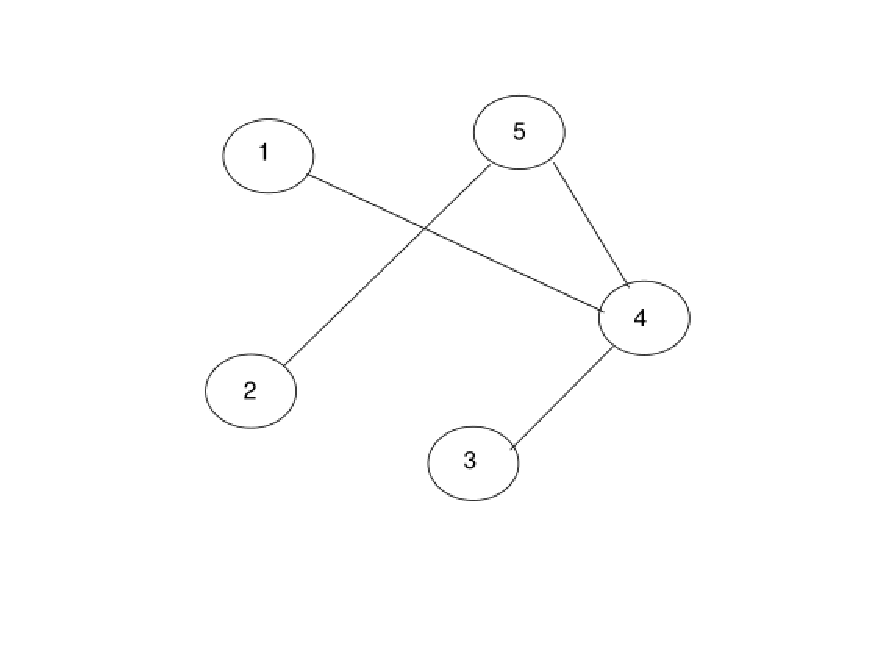
\includegraphics[width=1.8in]{delay/tuopu3.eps}}
     \end{center}
  \caption{网络系统在不同马氏链状态下可能的拓扑结构图.}\label{tuopu}
  \end{figure}
        本节给出一个数值的例子来印证定理的有效性. 考虑一个带有部分未知转移率和自身动力学时滞共存的马尔可夫切换耦合的复杂网络, 该网络包含$5$ 个节点, 每个节点包含$3$个状态, 其动力学方程如下:
        \begin{align}\label{numbersys}
           \nonumber \dot{x}_{i}(t)&=f(t,x_{i}(t),x_i(t-\tau))-c\sum^5_{j=1}l_{ij}(r_{t})[x_{j}(t_k)-x_{i}(t_{k})]+u_i(t),\\
            &\quad\quad t_{k}\leq t< t_{k+1} \quad i = 1,\cdots,5,
        \end{align}
        其中$x_i(t)=(x_{i}^{1}(t),x_{i}^{2}(t),x_{i}^{3}(t))^{\top}\in R^{n}$是第$i$个节点的状态向量; $f(t,x_{i}(t), x_i(t-\tau))=(-z(1+b)x_i^1(t)+zx_i^2(t)-zh(x_i^1(t)), x_i^1(t)-x_i^2(t)+x_i^3(t), -\eta x_i^2(t)-ex_i^3(t)-\eta\epsilon\sin(\nu x_i^1(t-\tau)))$, $h(x)=1/2(a-b)(|x+1|-|x-1|)$. $z=9.78, a=-1.4325, b=-0.7831, \eta=9.53, e=0.1636, \epsilon=0.2, \nu=0.5, \tau=0.02$. $\{r_t, t\geq0\}$是有限状态空间$S=\{1,2,3\}$上的马氏链, 部分未知转率矩阵如下:
    $$
          Q=\left(
            \begin{array}{ccc}
              -8 & ? & ? \\
              5 & -8 & 3 \\
              ? & ? & -8 \\
            \end{array}
          \right),
          $$
\begin{figure}[!htb]
\begin{minipage}[t]{0.48\linewidth}
\centering
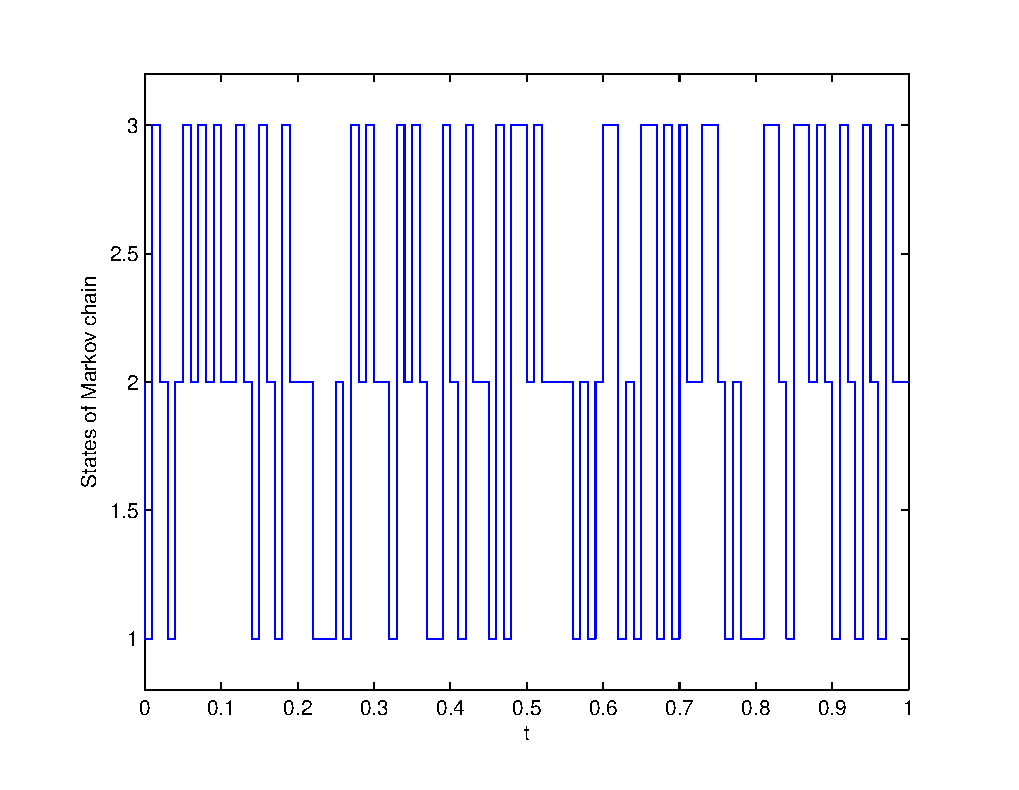
\includegraphics[width=3.2in]{delay/figure1.eps}
\caption{马尔可夫链$\{\sigma(t)|t\in[0,1]\}$在转移概率矩阵$Q$下的状态切换.}
\label{Markovfig}
\end{minipage}~~
\begin{minipage}[t]{0.48\linewidth}
\centering
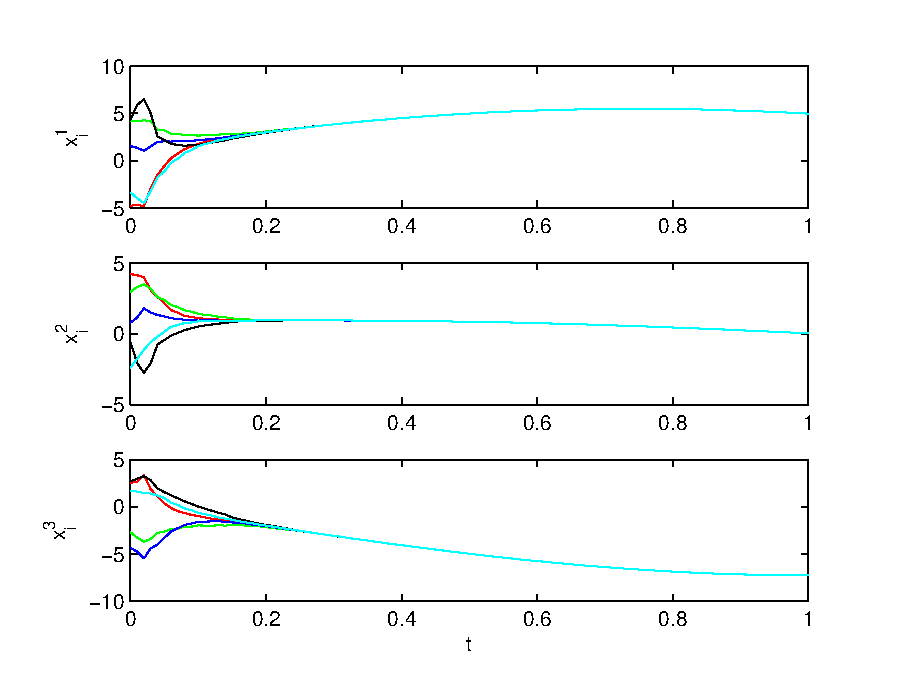
\includegraphics[width=3.2in]{delay/figure2.eps}
\caption{基于事件激发随机发生控制策略下, 时滞马氏系统 \eqref{numbersys} 在参数$c=8.2,\theta=20$下的节点状态向量轨道$x^j_i(t)(i=1,2,\cdots,5,j=1,2,3)$的变化情况.}
\label{state}
\end{minipage}
\end{figure}
\begin{figure}[!htb]
\begin{minipage}[t]{0.48\linewidth}
\centering
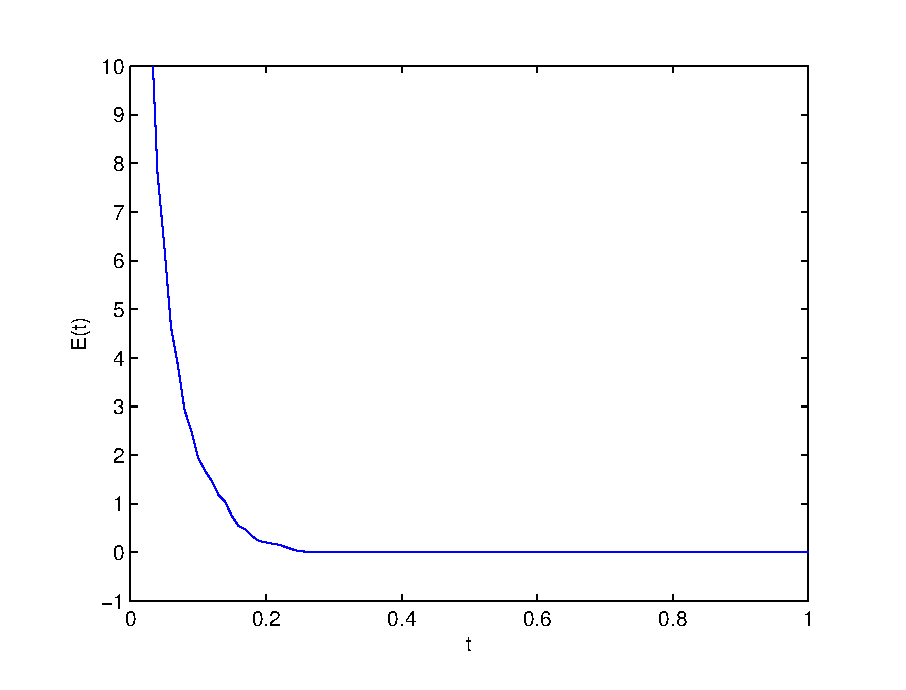
\includegraphics[width=3.2in]{delay/figure3.eps}
\caption{系统 \eqref{numbersys} 总同步误差轨道$E(t)$.}
\label{totallerror}
\end{minipage}~~
\begin{minipage}[t]{0.48\linewidth}
\centering
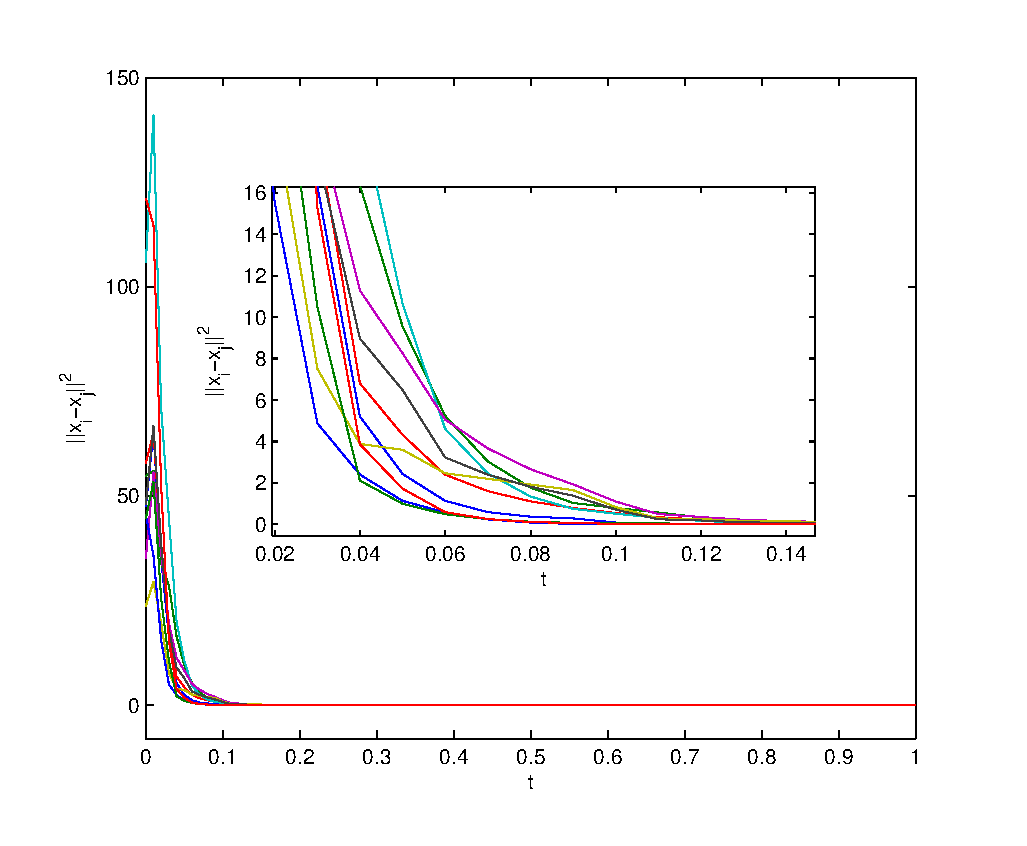
\includegraphics[width=3.2in,height=2.45in]{delay/xi-xj.eps}
\caption{不同节点间的状态差距$\|x_i-x_j\|^2, i=1,2,\cdots,5,j=i+1,i+2,\cdots,5$演变过程.}\label{xixj}
\end{minipage}
\end{figure}
    其中$"?"$表示未知的转移率. 可以看出, 马尔可夫链的平均逗留时间服从参数为$0.1$ 的指数分布, 并且$S_1^1=\{1\},S_2^1=\{2,3\},S_1^2=\{1,2,3\},S_2^2=\emptyset,S_1^3=\{3\},S_2^3=\{1,2\}$. 具体的演变过程见\autoref{Markovfig}.
    可能的耦合结构如\autoref{tuopu}.
$u_i(t)$是随机发生控制器, 其定义如下:
$$u_i(t)=-\rho c\beta_{i}(t)\frac{1}{N}\sum_{j=1}^N\Gamma[x_{i}(t_{k})-x_j(t_{k})],$$
其中$\rho c$是控制强度增益, $\{\beta_{i}(t), i=1,2,\cdots 5\}$是相互独立的随机过程, 并且满足$\mathrm{E}\{\beta_{i}(t)\}=0.8$.

下面验证\autoref{them} 与\autoref{them2} 的条件. 首先估计参数$\alpha_1$和$\alpha_2$使得$f(t,x(t),x(t-\tau))$满足\autoref{ass1}, 根据$f$的定义, 可以将$f$ 分解成时滞和非时滞两个部分: $f(t,x(t),x(t-\tau))=f_1(x(t))+f_2(x(t-\tau))$, 其中$f_1(x(t))=(-z(1+b)x_1(t)+zx_2(t)-zh(x_1(t)),x_1(t)-x_2(t)+x_3(t),-\eta x_2(t)-ex_3(t))^\top$, $f_2(x(t-\tau))=(0,0,-\eta\epsilon\sin(\nu x_1(t-\tau)))^\top$. 于是函数$f_1$所以可能的Jacobin矩阵为:
\begin{figure}[!htb]
\begin{minipage}[t]{0.48\linewidth}
\centering
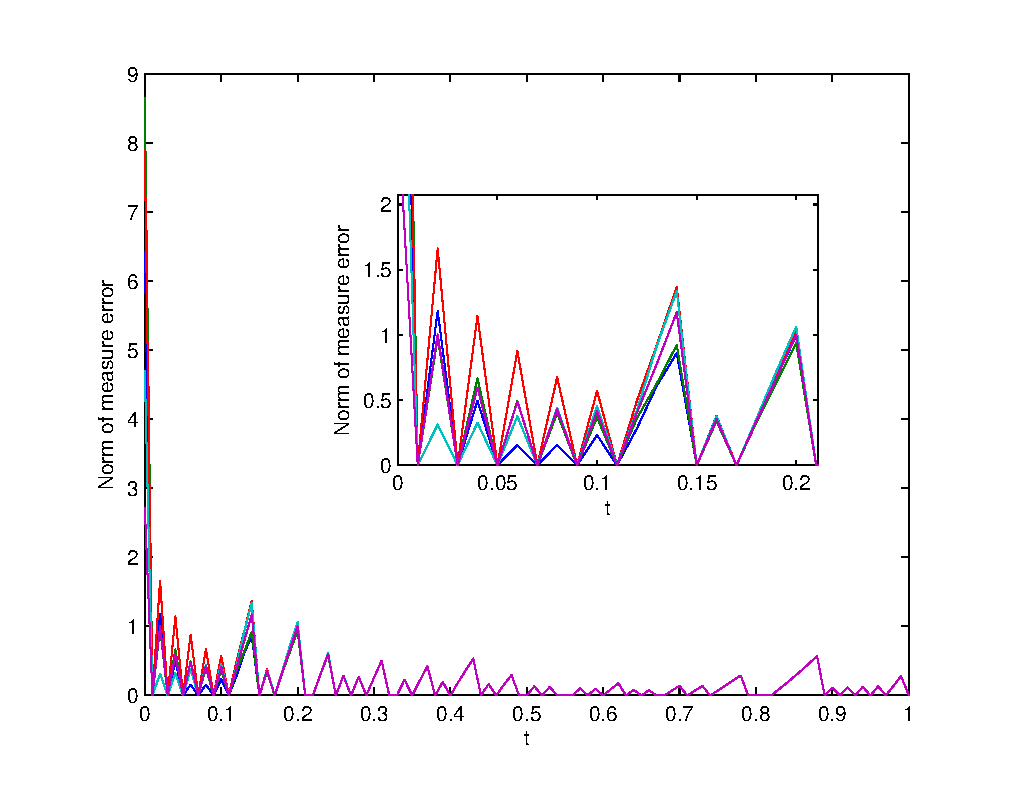
\includegraphics[width=3.2in]{delay/figure4.eps}
\caption{测量误差的变化过程.}
\label{measurerror}
\end{minipage}~~
\begin{minipage}[t]{0.48\linewidth}
\centering
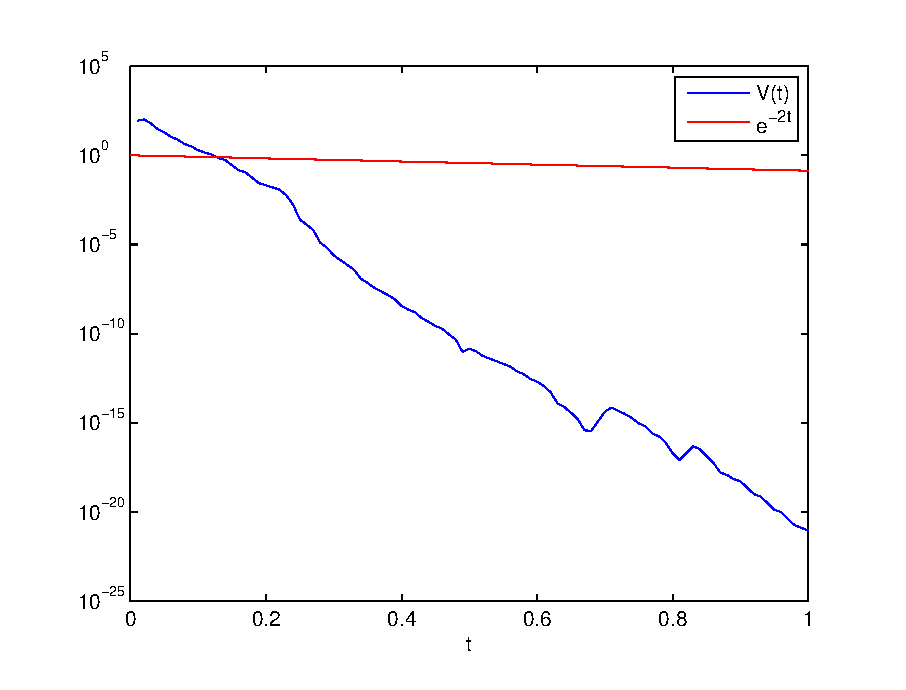
\includegraphics[width=3.2in,height=2.45in]{delay/figure5.eps}
\caption{Lyapunov-Krasovskii函数$V (t)$的变化过程.}\label{vt}
\end{minipage}
\end{figure}
       \begin{align*}
        J_1=\left(
              \begin{array}{ccc}
                4.2299 &  9.78 & 0 \\
                1 & -1 & 1 \\
                0 &  -9.53 & 0 \\
              \end{array}
            \right),
        J_2=\left(
              \begin{array}{ccc}
                -2.1213 & 9.78 & 0 \\
                1 & -1 & 1 \\
                0 &  -9.53 & 0 \\
              \end{array}
            \right).
        \end{align*}
        对于任意$x(t),x(t-\tau),y(t)$和$y(t-\tau)\in R^3$, 通过利用范数三角不等式性可得:
        \begin{align*}
        &\quad\|f(t,x(t),x(t-\tau))-f(t,y(t),y(t-\tau))\|\\
        &\leq\|f_1(x(t))-f_1(y(t))\|+\|f_2(x(t-\tau))-f_2(y(t-\tau))\|\\
        &=\max\{\|J_1\|,\|J_2\|\}\|(x(t)-y(t))\|
        +\|-\eta\epsilon\sin(\nu
            x_1(t-\tau))+\eta\epsilon\sin(\nu y_1(t-\tau))\|\\
        &\leq\max\{\|J_1\|,\|J_2\|\}\|(x(t)-y(t))\|
        +|\eta\epsilon\nu|\|x_1(t-\tau)-y_1(t-\tau)\|\\
        &\leq\max\{\|J_1\|,\|J_2\|\}\|(x(t)-y(t))\|
        +|\eta\epsilon\nu|\|x(t-\tau)-y(t-\tau)\|.
        \end{align*}
       因此取$\alpha_1=\max\{\|J_1\|,\|J_2\|\}=14.0228, \alpha_2=|\eta\epsilon\nu|=0.9530$可使得$f(t,x(t),x(t-\tau))$满足\autoref{ass1}.

 其次, 选取$a_1=17.39, a_2=-3$以及$a_3=20.08$, 则有$L^2_v-a_uI_N\leq 0(v\neq u, v\in S_2^u)$和$L^2_u-a_uI_N\geq 0(u\in S_2^u)$.
 最后, 选取$c=8.2, \rho=20, a=0.95$, 则有$\pi_1=23.66, \pi_2=28.822$, $\pi_3=27.94$以及$\varpi=0.35$. 容易证明, 对于任意$u\in\{1,2,3\}$$2a\lambda_2^2-\bar{\lambda}\alpha_2>0$且$\bar{\lambda}(\alpha_1\lambda^{-1}_2+\alpha_2)+a+\pi_u-c\gamma(\lambda_2+\rho\beta)<0$. 因此\autoref{them} 和\autoref{them2} 的条件满足.

 利用欧拉法, 取步长为$0.01$, 区间为$[0,1]$. 通过MATLAB求解微分方程 \eqref{numbersys} 并画出相应的变化图.

\autoref{Markovfig} 展现了在区间$[0,1]$马氏链在转移概率矩阵$Q$下的状态切换过程. \autoref{state} 描绘了网络节点的各个状态$x_i^j(t)(i=1,2,\cdots,5, j=1,2,3)$随着时间演变的过程, 从该图可以看出, 不同节点间的同一状态趋于同步. 即, 在事件激发随机发生控制策略下, 系统 \eqref{numbersys} 能够实现均方指数同步.

定义系统总误差如下:
        $$E(t)=\sqrt{\sum_{i=1}^5\sum_{j=1}^3\Big(x_i^j(t)-\frac{1}{5}\sum_{k=1}^5x_k^j(t)\Big)^2}.$$
系统总误差$E(t)$的演变过程参见\autoref{totallerror}. 各个节点轨道之间的距离差演变过程见\autoref{xixj}. 从\autoref{totallerror} 和\autoref{xixj} 可以看出, 网络系统 \eqref{numbersys} 在很短时间内达到同步. \autoref{measurerror} 描述了测量误差的演变过程, 从该图中可以看到, 测量误差线与横轴的角度就是事件激发的时刻, 图中任意两个激发时刻之间都存在间隔, 且间隔没有随着时间的延长而减小. 这说明事件激发时刻间隔的正下界是存在的, 即Zeno现象不会发生. \autoref{vt} 展示了Lyapunov—Krasovskii 函数$V (t)$的变化情况以及与指数函数$e^{-2t}$的对比, 可以看出, $V (t)$的收敛于零的速度比指数函数$e^{-2t}$快一些, 因此该同步属于指数同步.

\section{小结}\label{con}
     本章利用集中式事件激发采样策略和随机发生控制方法研究了动力学时滞和带有马氏切换耦合复杂网络同步问题. 网络的马氏链的转移率矩阵是部分未知的, 并且孤立节点动力学受到时滞的影响. 通过利用Lyapunov稳定性理论以及随机分析知识, 本章得出了充分的同步条件并保证了Zeno现象不会发生. 最后, 给出了一些数值的例子来证实结论的有效性.
